\setmodule{9}

%BEGIN_FOLD % ====>>_____ Занятие 1 _____<<====
\begin{class}[number=1]
	\begin{listofex}
		%11.2,3,4 по 3 первых
		\item Найдите точку максимума функции \(y=x^3-48x+17\).
		\item Найдите наименьшее значение функции \(y=x^3-27x\) на отрезке \([0;4]\).
		\item Найдите наибольшее значение функции \(y=x^3-3x+4\) на отрезке \([-2;0]\).
		\item Найдите точку максимума функции \(y=-\dfrac{ x^2+289 }{ x }\).
		\item Найдите точку минимума функции \(y=-\dfrac{ x^2+1 }{ x }\).
		\item Найдите наименьшее значение функции \(y=\dfrac{ x^2+25 }{ x }\) на отрезке \([1;10]\).
		\item Найдите наименьшее значение функции \(y=(x-8)e^{x-7}\) на отрезке \([6;8]\).
		\item Найдите точку минимума функции \(y=(x+16)e^{x-16}\).
		\item Найдите точку максимума функции \(y=(9-x)e^{x+9}\).
		\item Изюм получается в процессе сушки винограда. Сколько килограммов винограда потребуется для получения \(20\) килограммов изюма, если виноград содержит \(90\%\) воды, а изюм содержит \(5\%\) воды?
		%\item Изюм получается в процессе сушки винограда. Сколько килограммов винограда потребуется для получения \(16\) килограммов изюма, если виноград содержит \(90\%\) воды, а изюм содержит \(5\%\) воды?
		%BANK https://math-ege.sdamgia.ru/test?likes=99575 // https://math-ege.sdamgia.ru/test?likes=99576 // https://math-ege.sdamgia.ru/test?likes=99576 // https://math-ege.sdamgia.ru/test?likes=99578
		%по 2
		\item Имеется два сплава. Первый сплав содержит \(5\%\) меди, второй --- \(12\%\) меди. Масса второго сплава больше массы первого на \(9\) кг. Из этих двух сплавов получили третий сплав, содержащий \(10\%\) меди. Найдите массу третьего сплава. Ответ дайте в килограммах.
		%\item Имеется два сплава. Первый сплав содержит \(5\%\) меди, второй --- \(13\%\) меди. Масса второго сплава больше массы первого на \(9\) кг. Из этих двух сплавов получили третий сплав, содержащий \(10\%\) меди. Найдите массу третьего сплава. Ответ дайте в килограммах.
		
		\item Смешав \(11\)-процентный и \(72\)-процентный растворы кислоты и добавив \(10\) кг чистой воды, получили \(31\)-процентный раствор кислоты. Если бы вместо \(10\) кг воды добавили \(10\) кг \(50\)-процентного раствора той же кислоты, то получили бы \(51\)-процентный раствор кислоты. Сколько килограммов \(11\)-процентного раствора использовали для получения смеси?
		%\item Смешав \(55\)-процентный и \(97\)-процентный растворы кислоты и добавив \(10\) кг чистой воды, получили \(65\)-процентный раствор кислоты. Если бы вместо \(10\) кг воды добавили \(10\) кг \(50\)-процентного раствора той же кислоты, то получили бы \(75\)-процентный раствор кислоты. Сколько килограммов \(55\)-процентного раствора использовали для получения смеси?
		
		%\item Имеется два сплава. Первый содержит \(10\%\) никеля, второй --- \(35\%\) никеля. Из этих двух сплавов получили третий сплав массой \(150\) кг, содержащий \(30\%\) никеля. На сколько килограммов масса первого сплава была меньше массы второго?
		\item Имеется два сплава. Первый содержит \(15\%\) никеля, второй --- \(35\%\) никеля. Из этих двух сплавов получили третий сплав массой \(140\) кг, содержащий \(30\%\) никеля. На сколько килограммов масса первого сплава была меньше массы второго?
		
		
		\item Имеются два сосуда. Первый содержит \(30\) кг, а второй --- \(15\) кг раствора кислоты различной концентрации. Если эти растворы смешать, то получится раствор, содержащий \(34\%\) кислоты. Если же смешать равные массы этих растворов, то получится раствор, содержащий \(46\%\) кислоты. Сколько килограммов кислоты содержится в первом сосуде?
		%\item Имеются два сосуда. Первый содержит \(100\) кг, а второй --- \(20\) кг раствора кислоты различной концентрации. Если эти растворы смешать, то получится раствор, содержащий \(67\%\) кислоты. Если же смешать равные массы этих растворов, то получится раствор, содержащий \(77\%\) кислоты. Сколько килограммов кислоты содержится в первом сосуде?
	\end{listofex}
\end{class}
%END_FOLD

%BEGIN_FOLD % ====>>_____ Занятие 2 _____<<====
\begin{class}[number=2]
	\begin{listofex}
		%11.2,3 по 4-5 И 11.4 3 первых
		\item Найдите точку максимума функции \(y=x^3-3x^2+2\).
		\item Найдите точку минимума функции \(y=2x^3-5x^2+1\).
		\item Найдите наибольшее значение функции \(y=\dfrac{ x^2+25 }{ x }\) на отрезке \([-10;-1]\).
		\item Найдите точку максимума функции \(y=\dfrac{ 16 }{x  }+x+3\).
		\item Найдите наименьшее значение функции \(y=(x-8)e^{x-7}\) на отрезке \([6;8]\).
		\item Найдите точку минимума функции \(y=(x+16)e^{x-16}\).
		\item Найдите точку максимума функции \(y=(9-x)e^{x+9}\).
		%по 2
		\item Имеется два сплава. Первый сплав содержит \(5\%\) меди, второй --- \(12\%\) меди. Масса второго сплава больше массы первого на \(9\) кг. Из этих двух сплавов получили третий сплав, содержащий \(10\%\) меди. Найдите массу третьего сплава. Ответ дайте в килограммах.
		%\item Имеется два сплава. Первый сплав содержит \(5\%\) меди, второй --- \(13\%\) меди. Масса второго сплава больше массы первого на \(9\) кг. Из этих двух сплавов получили третий сплав, содержащий \(10\%\) меди. Найдите массу третьего сплава. Ответ дайте в килограммах.
		
		\item Смешав \(11\)-процентный и \(72\)-процентный растворы кислоты и добавив \(10\) кг чистой воды, получили \(31\)-процентный раствор кислоты. Если бы вместо \(10\) кг воды добавили \(10\) кг \(50\)-процентного раствора той же кислоты, то получили бы \(51\)-процентный раствор кислоты. Сколько килограммов \(11\)-процентного раствора использовали для получения смеси?
		%\item Смешав \(55\)-процентный и \(97\)-процентный растворы кислоты и добавив \(10\) кг чистой воды, получили \(65\)-процентный раствор кислоты. Если бы вместо \(10\) кг воды добавили \(10\) кг \(50\)-процентного раствора той же кислоты, то получили бы \(75\)-процентный раствор кислоты. Сколько килограммов \(55\)-процентного раствора использовали для получения смеси?
		
		%\item Имеется два сплава. Первый содержит \(10\%\) никеля, второй --- \(35\%\) никеля. Из этих двух сплавов получили третий сплав массой \(150\) кг, содержащий \(30\%\) никеля. На сколько килограммов масса первого сплава была меньше массы второго?
		\item Имеется два сплава. Первый содержит \(15\%\) никеля, второй --- \(35\%\) никеля. Из этих двух сплавов получили третий сплав массой \(140\) кг, содержащий \(30\%\) никеля. На сколько килограммов масса первого сплава была меньше массы второго?
		
		
		\item Имеются два сосуда. Первый содержит \(30\) кг, а второй --- \(15\) кг раствора кислоты различной концентрации. Если эти растворы смешать, то получится раствор, содержащий \(34\%\) кислоты. Если же смешать равные массы этих растворов, то получится раствор, содержащий \(46\%\) кислоты. Сколько килограммов кислоты содержится в первом сосуде?
		%\item Имеются два сосуда. Первый содержит \(100\) кг, а второй --- \(20\) кг раствора кислоты различной концентрации. Если эти растворы смешать, то получится раствор, содержащий \(67\%\) кислоты. Если же смешать равные массы этих растворов, то получится раствор, содержащий \(77\%\) кислоты. Сколько килограммов кислоты содержится в первом сосуде?
	\end{listofex}
\end{class}
%END_FOLD

%BEGIN_FOLD % ====>>_ Домашняя работа 1 _<<====
\begin{homework}[number=1]
	\begin{listofex}
		%11.2,3 по 6-7 И 11.4 4-5
		\item Найдите наименьшее значение функции \(y=x^3-3x^2+2\) на отрезке \([1;4]\).
		\item Найдите наибольшее значение функции \(y=x^3-6x^2\) на отрезке \([-3;3]\).
		\item Найдите точку минимума функции \(y=\dfrac{ 25 }{ x }+x+25\).
		\item Найдите точку максимума функции \(y=-\dfrac{ x }{ x^2+9 }\).
		\item Найдите точку минимума функции \(y=(3-x)e^{3-x}\).
		\item Найдите наибольшее значение функции \(y=(x+16)e^{16-x}\) на отрезке \([15;17]\).
		\item Изюм получается в процессе сушки винограда. Сколько килограммов винограда потребуется для получения \(82\) килограммов изюма, если виноград содержит \(90\%\) воды, а изюм содержит \(5\%\) воды?
		\item Два промышленных фильтра, работая одновременно, очищают цистерну воды за \(30\) минут. Определите, за сколько минут второй фильтр очистит цистерну воды, работая отдельно, если известно, что он сделает это на \(25\) минут быстрее, чем первый.
	\end{listofex}
\end{homework}
%END_FOLD

%BEGIN_FOLD % ====>>_____ Занятие 3 _____<<====
\begin{class}[number=3]
	\begin{listofex}
		%11.4 7-9 И 11.5 1-4
		\item Найдите точку максимума функции \( y=(3x^2-36x+36)e^{x+36}. \)
		\item Найдите точку максимума функции \(y=(x^2-10x+10)e^{5-x}\).
		\item Найдите точку максимума функции \(y=(x-2)^2e^{x-6}\).
		\item Найдите наибольшее значение функции \(y=8\ln(x+7)-8x+3\) на отрезке \([-6,5; 0]\).
		\item Найдите наименьшее значение функции \(y=4x-4\ln(x+7)+6\) на отрезке \([-6,5; 0]\).
		\item Найдите наибольшее значение функции \(y=\ln(x+5)^5-5x\) на отрезке \([-4,5; 0]\).
		\item Найдите наименьшее значение функции \(y=3x-\ln(x+3)^3\) на отрезке \([-2,5; 0]\).
		
		
		
		%BANK https://math-ege.sdamgia.ru/test?likes=99575 // https://math-ege.sdamgia.ru/test?likes=99576 // https://math-ege.sdamgia.ru/test?likes=99576 // https://math-ege.sdamgia.ru/test?likes=99578
		%по 2
		\item Имеется два сплава. Первый сплав содержит \(5\%\) меди, второй --- \(12\%\) меди. Масса второго сплава больше массы первого на \(9\) кг. Из этих двух сплавов получили третий сплав, содержащий \(10\%\) меди. Найдите массу третьего сплава. Ответ дайте в килограммах.
		%\item Имеется два сплава. Первый сплав содержит \(5\%\) меди, второй --- \(13\%\) меди. Масса второго сплава больше массы первого на \(9\) кг. Из этих двух сплавов получили третий сплав, содержащий \(10\%\) меди. Найдите массу третьего сплава. Ответ дайте в килограммах.
		
		\item Смешав \(11\)-процентный и \(72\)-процентный растворы кислоты и добавив \(10\) кг чистой воды, получили \(31\)-процентный раствор кислоты. Если бы вместо \(10\) кг воды добавили \(10\) кг \(50\)-процентного раствора той же кислоты, то получили бы \(51\)-процентный раствор кислоты. Сколько килограммов \(11\)-процентного раствора использовали для получения смеси?
		
		
		%\item Имеется два сплава. Первый содержит \(10\%\) никеля, второй --- \(35\%\) никеля. Из этих двух сплавов получили третий сплав массой \(150\) кг, содержащий \(30\%\) никеля. На сколько килограммов масса первого сплава была меньше массы второго?
		
		%\item Имеются два сосуда. Первый содержит \(100\) кг, а второй --- \(20\) кг раствора кислоты различной концентрации. Если эти растворы смешать, то получится раствор, содержащий \(67\%\) кислоты. Если же смешать равные массы этих растворов, то получится раствор, содержащий \(77\%\) кислоты. Сколько килограммов кислоты содержится в первом сосуде?
	\end{listofex}
\end{class}
%END_FOLD

%BEGIN_FOLD % ====>>_____ Занятие 4 _____<<====
\begin{class}[number=4]
	\begin{listofex}
		%%11.4 10-13 И 11.5 5-8 И 11.6 1-3
		%\item Найдите точку минимума функции \( y=(x-2)^2 e^{ x-5} \).
		%\item Найдите точку максимума функции \( y=(x+6)^2 e^{4-x} \).
		%\item Найдите точку минимума функции \( y=(x+3)^2e^{2-x} \).
		%\item Найдите точку минимума функции \(y=(x^2-8x+8)e^{6-x}\).
		%\item Найдите наименьшее значение функции \( y=9x-\ln(9x)+3 \) на отрезке \(\left[ \dfrac{1  }{ 18 }; \dfrac{ 5 }{ 18 } \right] \).
		%\item Найдите наибольшее значение функции \( y=\ln(11x)-11x+9 \) на отрезке \(\left[ \dfrac{ 1 }{ 22}; \dfrac{ 5 }{ 22 } \right] \).
		%\item Найдите наибольшее значение функции \( y=2x^2-13x+9\ln x + 8 \) на отрезке \(\left[ \dfrac{ 13 }{ 14 }; \dfrac{15  }{14  } \right] \).
		%\item Найдите наименьшее значение функции \( y=2x^2-5x+\ln x-3 \) на отрезке \(\left[ \dfrac{ 5 }{ 6 }; \dfrac{ 7 }{ 6 } \right] \).
		%
		
		%
		
		%525690
		\item
		\begin{minipage}[t]{\bodywidth}
			На рисунке изображены график функции \(y=f(x)\) и касательная к этому графику, проведённая в точке \(x_0\). Уравнение касательной показано на рисунке. Найдите значение производной функции \(g(x)=-7f(x)+21x+\dfrac{ 1 }{ 441 }\) в точке \(x_0\).
		\end{minipage}
		\hspace{0.02\linewidth}
		\begin{minipage}[t]{\picwidth}
			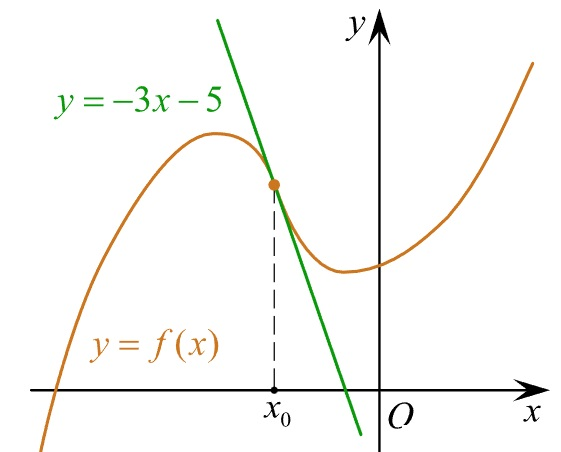
\includegraphics[align=t, width=\linewidth]{\picpath/G112M8C3-1}
		\end{minipage}
		%525702
		\item
		\begin{minipage}[t]{\bodywidth}
			На рисунке изображены график функции \(y=f(x)\) и касательная к этому графику, проведённая в точке \(x_0\). Уравнение касательной показано на рисунке. Найдите значение производной функции \(g(x)=-5f(x)-\dfrac{ 2 }{ 11 }x+\ln3\) в точке \(x_0\).
		\end{minipage}
		\hspace{0.02\linewidth}
		\begin{minipage}[t]{\picwidth}
			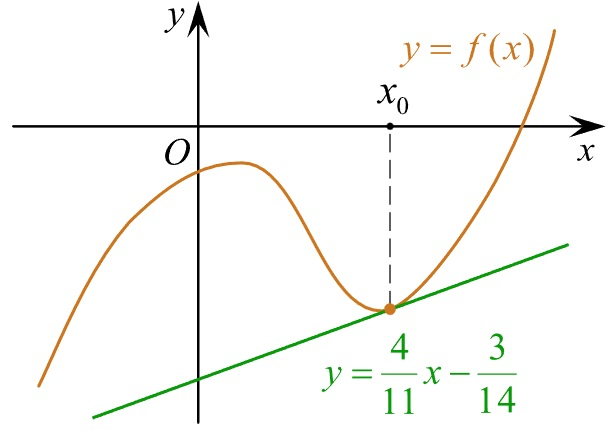
\includegraphics[align=t, width=\linewidth]{\picpath/G112M8C3-2}
		\end{minipage}
		%525691
		\item
		\begin{minipage}[t]{\bodywidth}
			На рисунке изображены график функции \(y=f(x)\) и касательная к этому графику, проведённая в точке \(x_0\). Уравнение касательной показано на рисунке. Найдите значение производной функции \(g(x)=(f'(x)-0,5)\cdot 6\) в точке \(x_0\).
		\end{minipage}
		\hspace{0.02\linewidth}
		\begin{minipage}[t]{\picwidth}
			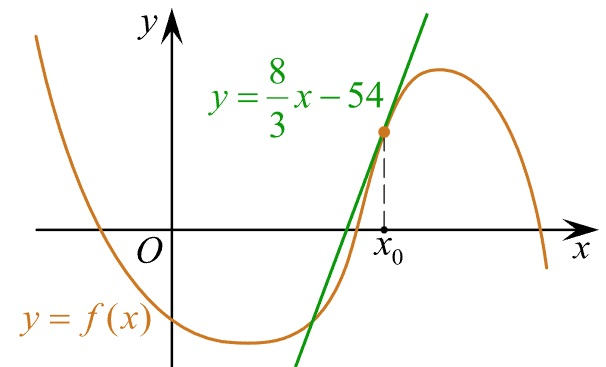
\includegraphics[align=t, width=\linewidth]{\picpath/G112M8C3-3}
		\end{minipage}
		%525703
		\item
		\begin{minipage}[t]{\bodywidth}
			На рисунке изображены график функции \(y=f(x)\) и касательная к этому графику, проведённая в точке \(x_0\). Уравнение касательной показано на рисунке. Найдите значение производной функции \(g(x)=f'(x)-f(x)+3\) в точке \(x_0\).
		\end{minipage}
		\hspace{0.02\linewidth}
		\begin{minipage}[t]{\picwidth}
			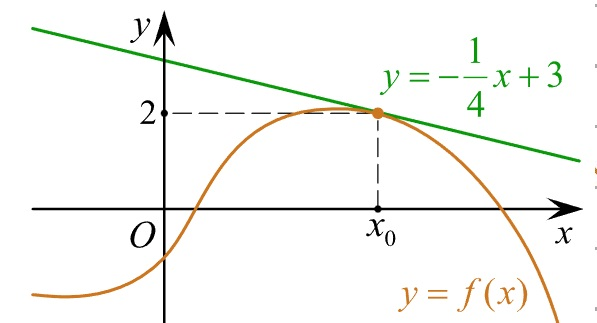
\includegraphics[align=t, width=\linewidth]{\picpath/G112M8C3-4}
		\end{minipage}
		%541816
		\item
		\begin{minipage}[t]{\bodywidth}
			На рисунке изображены график функции \(y=f(x)\) и касательная к нему в точке с абсциссой \(x_0\). Найдите значение производной функции \(f(x)\)в точке \(x_0\).
		\end{minipage}
		\hspace{0.02\linewidth}
		\begin{minipage}[t]{\picwidth}
			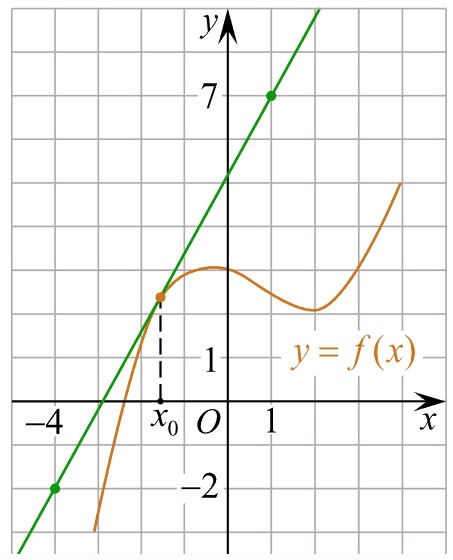
\includegraphics[align=t, width=\linewidth]{\picpath/maksutovM8L4-1}
		\end{minipage}
		%9063
		\item
		\begin{minipage}[t]{\bodywidth}
			На рисунке изображены график функции \(y=f(x)\) и касательная к нему в точке с абсциссой \(x_0\). Найдите значение производной функции \(f(x)\)в точке \(x_0\).
		\end{minipage}
		\hspace{0.02\linewidth}
		\begin{minipage}[t]{\picwidth}
			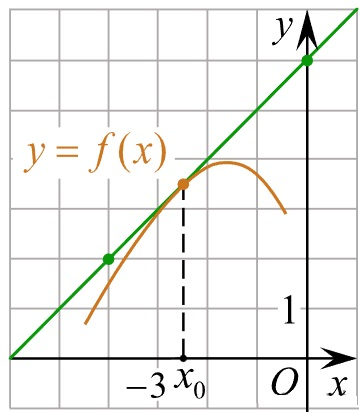
\includegraphics[align=t, width=\linewidth]{\picpath/maksutovM8L4-2}
		\end{minipage}
		%9629
		\item
		\begin{minipage}[t]{\bodywidth}
			На рисунке изображены график функции \(y=f(x)\) и касательная к нему в точке с абсциссой \(x_0\). Найдите значение производной функции \(f(x)\)в точке \(x_0\).
		\end{minipage}
		\hspace{0.02\linewidth}
		\begin{minipage}[t]{\picwidth}
			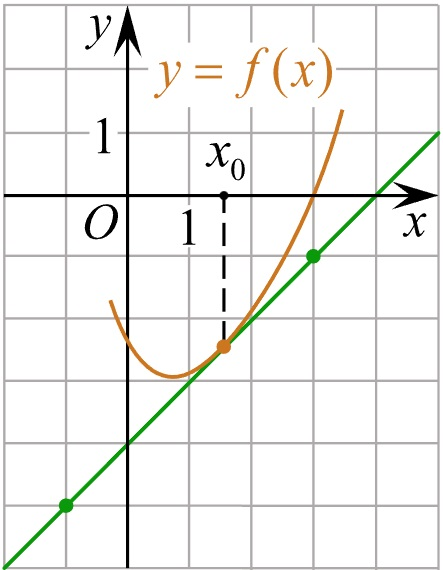
\includegraphics[align=t, width=\linewidth]{\picpath/maksutovM8L4-3}
		\end{minipage}
		
		
		%11-1M8L1 до 6 номера
		\item Вычислить:
		\begin{tasks}(2)
			\task \( \dfrac{-13\sin126\degree}{\sin54\degree} \)
			\task \( \cos^2(-46\degree)+\sin^2(-46\degree) \)
			\task \( \sin^223\degree+9+\cos^223 \)
			\task \( \dfrac{2\sin^221\degree+2\cos^221\degree}{4} \)
		\end{tasks}
		\item Найдите значение выражения: \( \sin\left( \dfrac{\pi}{3}+\alpha \right) \), если \( \cos\alpha=-\dfrac{8}{17} \) и \\ \( \pi<\alpha<\dfrac{3\pi}{2} \).
		%G111M87L2N3
		\item Найдите: %101L1
		\begin{tasks}
			
			\task \( -2\sin\alpha \), если \( \cos\alpha=\dfrac{\sqrt{6}}{5} \) и \( \alpha\in\left( \dfrac{\pi}{2}; \pi \right) \);
			\task \( -\cos\alpha \), если \( \sin\alpha=-\dfrac{5\sqrt{2}}{8} \) и \( \alpha\in\left( \dfrac{3\pi}{2}; 2\pi \right) \);
			\task \( -5\cos\alpha \), если \( \sin\alpha=0,6 \);
			\task \( \sin\left( \dfrac{3\pi}{2}+\alpha \right) \), если \( \sin\alpha=0,6 \) и \( \alpha\in\left( \dfrac{\pi}{2}; \pi \right) \).
		\end{tasks}
		
		\item Найдите наибольшее значение функции \( y=12 \cos x + 6 \sqrt{3} x -2 \sqrt{3} \pi + 6 \) на отрезке \(\left[ 0;\dfrac{ \pi }{ 2 } \right] \).
		\item Найдите наименьшее значение функции \( y=3+\dfrac{5\pi  }{4  }-5x-5\sqrt{2} \cos x \) на отрезке \(\left[ 0; \dfrac{ \pi }{ 2 } \right] \).
		\item Найдите наибольшее значение функции \( y=5 \cos x -6x+4 \) на отрезке \(\left[ -\dfrac{3\pi  }{ 2 };0 \right] \).
		
	\end{listofex}
\end{class}
%END_FOLD

%BEGIN_FOLD % ====>>_ Домашняя работа 2 _<<====
\begin{homework}[number=2]
	\begin{listofex}
		%G111M8L5
		%analog 26784 1-2 V 62785 1-2
		\item Найдите:
		\begin{tasks}
			\task \( -2 \sin \left( \dfrac{ \pi }{ 2 }+\alpha \right) \), если \( \sin \alpha = -0,96 \) и \( \alpha \in (\pi;1,5\pi) \);
			\task \( -4 \cos \left( \dfrac{ 5\pi }{ 2 }+ \alpha \right) \), если \( \cos \alpha = \dfrac{ 7 }{ 25 } \) и \( \alpha \in (1,5\pi; 2\pi) \);
			\task \( 2\sin \left( \dfrac{ \pi }{ 2 }- \alpha \right) \), если \( \sin \alpha = -0,8 \) и \( \alpha \in (1,5\pi;2\pi) \);
			\task \( 5 \cos \left( \dfrac{ 7\pi }{ 2 } + \alpha \right) \), если \( \cos \alpha = \dfrac{ \sqrt{2} }{ 2 } \) и \( \alpha \in (0;0,5\pi) \).
		\end{tasks}
		%11 trigon 4-7
		\item Найдите наибольшее значение функции \( y=15x-3\sin x+5 \) на отрезке \(\left[ -\dfrac{ \pi }{ 2 };0 \right] \).
		\item Найдите наименьшее значение функции \( y=9\cos x +14x +7 \) на отрезке \(\left[ 0;\dfrac{ 3\pi }{ 2 } \right] \).
		\item Найдите наименьшее значение функции \( y=7 \sin x -8x +9 \) на отрезке \(\left[ -\dfrac{ 3\pi }{ 2 };0 \right] \).
		\item Найдите наименьшее значение функции \( y=6 \cos x + \dfrac{ 24 }{ \pi }x+5 \) на отрезке \(\left[ -\dfrac{ 2\pi }{ 3 };0 \right] \).
		%11.5 5-7
		\item Найдите наибольшее значение функции \( y=9x-\ln(9x)+3 \) на отрезке \(\left[ \dfrac{ 1 }{ 18 };\dfrac{ 5 }{ 18 } \right] \).
		\item Найдите наибольшее значение функции \( y=\ln(11x)-11x+9 \) на отрезке \(\left[ \dfrac{ 1 }{ 22 };\dfrac{5  }{22  } \right] \).
		\item Найдите наибольшее значение функции \( y=2x^2-13x+9 \ln x +8 \) на отрезке \(\left[ \dfrac{ 13 }{ 14 }; \dfrac{  15}{ 14 } \right] \).
		%\item Найдите наибольшее значение функции \(  \) на отрезке \(\left[  \right] \).
		%\item Смешав \(55\)-процентный и \(97\)-процентный растворы кислоты и добавив \(10\) кг чистой воды, получили \(65\)-процентный раствор кислоты. Если бы вместо \(10\) кг воды добавили \(10\) кг \(50\)-процентного раствора той же кислоты, то получили бы \(75\)-процентный раствор кислоты. Сколько килограммов \(55\)-процентного раствора использовали для получения смеси?
		\item Имеется два сплава. Первый содержит \(15\%\) никеля, второй --- \(35\%\) никеля. Из этих двух сплавов получили третий сплав массой \(140\) кг, содержащий \(30\%\) никеля. На сколько килограммов масса первого сплава была меньше массы второго?
		%9629
		\item
		\begin{minipage}[t]{\bodywidth}
			На рисунке изображены график функции \(y=f(x)\) и касательная к нему в точке с абсциссой \(x_0\). Найдите значение производной функции \(f(x)\)в точке \(x_0\).
		\end{minipage}
		\hspace{0.02\linewidth}
		\begin{minipage}[t]{\picwidth}
			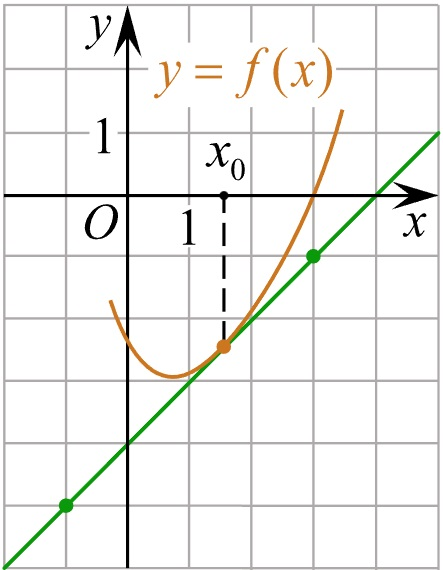
\includegraphics[align=t, width=\linewidth]{\picpath/maksutovM8L4-3}
		\end{minipage}
		%\item 
		%\begin{minipage}[t]{0.45\linewidth}
		%	На рисунке изображены график функции \( y=f(x) \) и касательная к этому графику, проведённая в точке \( x_0=2 \). Найдите значение производной функции \( g(x)=x^2-f(x)+1 \) в точке \( x_0 \).
		%\end{minipage}
		%\begin{minipage}[t]{0.5\linewidth}
		%	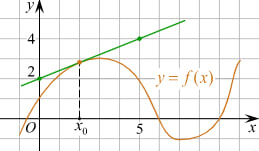
\includegraphics[align=t, width=\textwidth]{\picpath/KuznetsovM8L2_1}
		%\end{minipage}
		%9641
		\item
		\begin{minipage}[t]{0.45\linewidth}
			На рисунке изображены график функции \(y=f(x)\) и касательная к этому графику, проведённая в точке \(x_0\). Уравнение касательной показано на рисунке. Найдите значение производной функции \(g(x)=12f(x)+\dfrac{  6}{13  }\) в точке \(x_0\).
		\end{minipage}
		\hspace{0.02\linewidth}
		\begin{minipage}[t]{0.5\linewidth}
			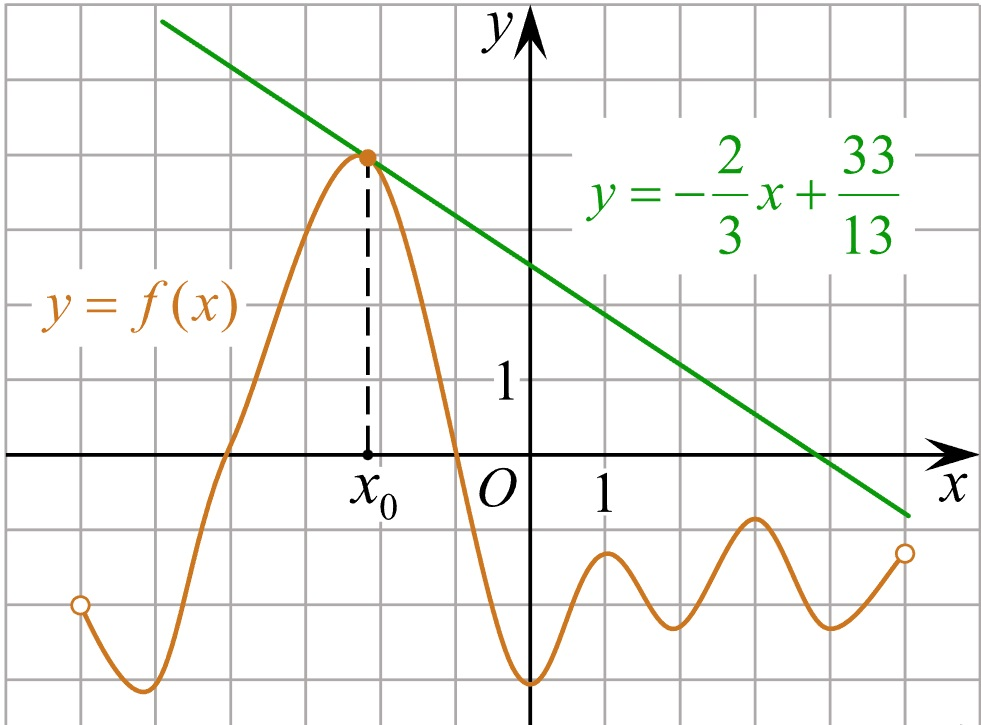
\includegraphics[align=t, width=\linewidth]{\picpath/G111M9H2-1}
		\end{minipage}
		%525446
		%\item
		%\begin{minipage}[t]{0.45\linewidth}
		%	На рисунке изображён график функции \(y=f(x)\) и касательная к нему в точке с абсциссой \(x_0\). Найдите значение производной функции \(f(x)\) в точке \(x_0\).
		%\end{minipage}
		%\hspace{0.02\linewidth}
		%\begin{minipage}[t]{0.5\linewidth}
		%	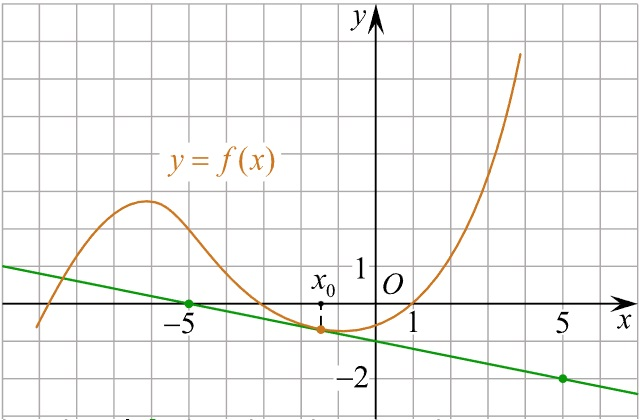
\includegraphics[align=t, width=\linewidth]{\picpath/maksutovM9L2-3}
		%\end{minipage}
		%%525401
		%\item
		%\begin{minipage}[t]{0.45\linewidth}
		%	На рисунке изображён график функции \(y=f(x)\) и касательная к нему в точке с абсциссой \(x_0\). Найдите значение производной функции \(f(x)\) в точке \(x_0\).
		%\end{minipage}
		%\hspace{0.02\linewidth}
		%\begin{minipage}[t]{0.5\linewidth}
		%	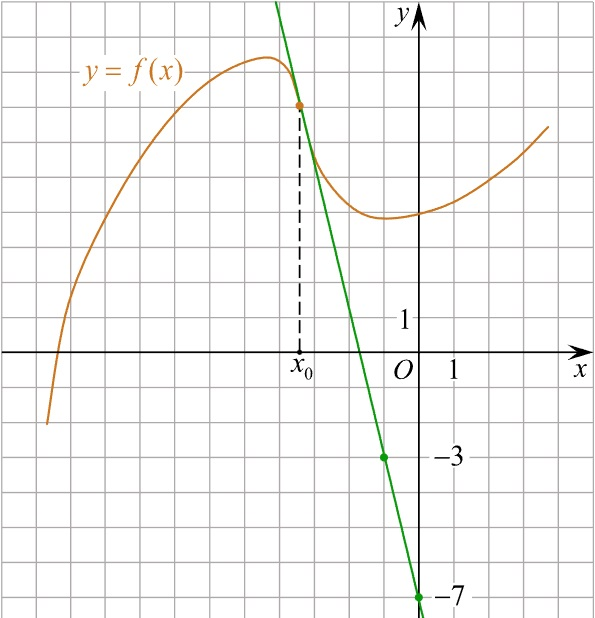
\includegraphics[align=t, width=\linewidth]{\picpath/maksutovM9L2-2}
		%\end{minipage}
		%\item Имеются два сосуда. Первый содержит \(30\) кг, а второй --- \(15\) кг раствора кислоты различной концентрации. Если эти растворы смешать, то получится раствор, содержащий \(34\%\) кислоты. Если же смешать равные массы этих растворов, то получится раствор, содержащий \(46\%\) кислоты. Сколько килограммов кислоты содержится в первом сосуде?
	\end{listofex}
\end{homework}
%END_FOLD

%BEGIN_FOLD % ====>>_____ Занятие 5 _____<<====
\begin{class}[number=5]
	\begin{listofex}
		\item Основания равнобедренной трапеции равны \(51\) и \(65\). Боковые стороны равны \(25\). Найдите синус острого угла трапеции.
		\item Основания равнобедренной трапеции равны \(43\) и \(73\). Косинус острого угла трапеции равен \(\dfrac{  5}{ 7 }\).  Найдите боковую сторону.
		\item Меньшее основание равнобедренной трапеции равно \(23\). Высота трапеции равна \(39\). Тангенс острого угла равен \(\dfrac{ 13 }{ 8 }\). Найдите большее основание.
		\item Основания равнобедренной трапеции равны \(14\) и \(26\), а ее периметр равен \(60\). Найдите площадь трапеции.
		\item Найдите площадь прямоугольной трапеции, основания которой равны \(6\) и \(2\), большая боковая сторона составляет с основанием угол \(45\degree \).
		\item Основания трапеции равны \(18\) и \(6\), боковая сторона, равная \(7\), образует с одним из оснований трапеции угол \(150\degree \). Найдите площадь трапеции.
		\item Основания трапеции равны \(27\) и \(9\), боковая сторона равна \(8\). Площадь трапеции равна \(72\). Найдите острый угол трапеции, прилежащий к данной боковой стороне. Ответ выразите в градусах.
		\item Чему равен больший угол равнобедренной трапеции, если известно, что разность противолежащих углов равна \(50\degree \)? Ответ дайте в градусах.
		\item Средняя линия трапеции равна \(28\), а меньшее основание равно \(18\). Найдите большее основание трапеции.
		\item В равнобедренной трапеции большее основание равно \(25\), боковая сторона равна \(10\), угол между ними \(60\) градусов. Найдите меньшее основание.
		\item
		\begin{minipage}[t]{\bodywidth}
			Через концы \(A, B\) дуги окружности в \(62\degree \) проведены касательные \(AC\) и \(BC\). Найдите угол \(ACB\). Ответ дайте в градусах.
		\end{minipage}
		\hspace{0.02\linewidth}
		\begin{minipage}[t]{\picwidth}
			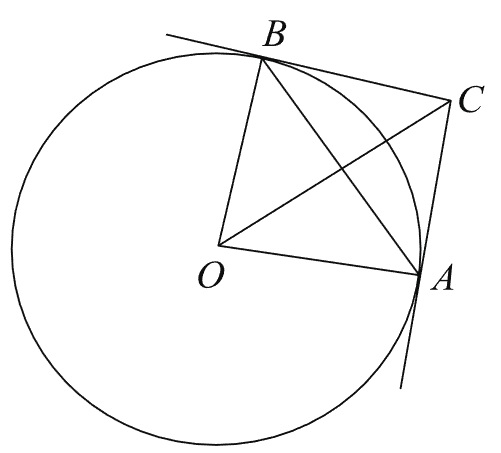
\includegraphics[align=t, width=\linewidth]{\picpath/MECGERM9H2-5}
		\end{minipage}
		\item Треугольник \(ABC\) вписан в окружность с центром \(O\). Найдите угол \(BOC\), если угол \(BAC\) равен \(32\degree \).
		\item Найдите центральный угол \(AOB\), если он на \(15\degree \) больше вписанного угла \(ACB\), опирающегося на ту же дугу. Ответ дайте в градусах.
		\item Периметр треугольника равен \(12\), а радиус вписанной окружности равен \(1\). Найдите площадь этого треугольника.
		
		
		
		
	\end{listofex}
\end{class}
%END_FOLD

%BEGIN_FOLD % ====>>_____ Занятие 6 _____<<====
\begin{class}[number=6]
	\begin{listofex}
		\item Занятие 6
	\end{listofex}
\end{class}
%END_FOLD

%BEGIN_FOLD % ====>>_ Домашняя работа 3 _<<====
\begin{homework}[number=3]
	\begin{listofex}
		\item Основания равнобедренной трапеции равны \(15\) и \(20\), а ее боковые стороны равны \(10\). Найдите площадь трапеции.
		\item Перпендикуляр, опущенный из вершины тупого угла на большее основание равнобедренной трапеции, делит его на части, имеющие длины \(10\) и \(4\). Найдите среднюю линию этой трапеции.
		\item Найдите площадь прямоугольной трапеции, основания которой равны \(5\) и \(10\), большая боковая сторона составляет с основанием угол \(30\degree \).
		\item В равнобедренной трапеции большее основание равно \(15\), боковая сторона равна \(4\), угол между ними \(45\) градусов. Найдите меньшее основание.
		\item Основания равнобедренной трапеции равны \(6\) и \(12\). Синус острого угла трапеции равен \(0,8\). Найдите боковую сторону.
		\item Точки \(A, B, C\), расположенные на окружности, делят ее на три дуги, градусные величины которых относятся как \(1 : 3 : 5\). Найдите больший угол треугольника \(ABC\). Ответ дайте в градусах.
		\item Радиус окружности, описанной около правильного треугольника, равен \(3\). Найдите высоту этого треугольника.
	\end{listofex}
\end{homework}
%END_FOLD

%BEGIN_FOLD % ====>>_____ Занятие 7 _____<<====
\begin{class}[number=7]
	\begin{listofex}
		\item Найдите радиус окружности, вписанной в правильный треугольник, высота которого равна \(6\).
		\item Сторона правильного треугольника равна \(\sqrt{3}\). Найдите радиус окружности, описанной около этого треугольника.
		\item Найдите сторону правильного шестиугольника, описанного около окружности, радиус которой равен \(\sqrt{3}\).
		\item Чему равна сторона правильного шестиугольника, вписанного в окружность, радиус которой равен \(6\)?
		\item Даны два шара. Радиус первого шара в \(2\) раза больше радиуса второго. Во сколько раз площадь поверхности первого шара больше площади поверхности второго?
		\item Шар вписан в цилиндр. Площадь полной поверхности цилиндра равна \(18\). Найдите площадь поверхности шара.
		
		\item
		\begin{minipage}[t]{\bodywidth}
			Найдите сторону правильного шестиугольника, описанного около окружности, радиус которой равен \(\sqrt{3}\).
		\end{minipage}
		\hspace{0.02\linewidth}
		\begin{minipage}[t]{\picwidth}
			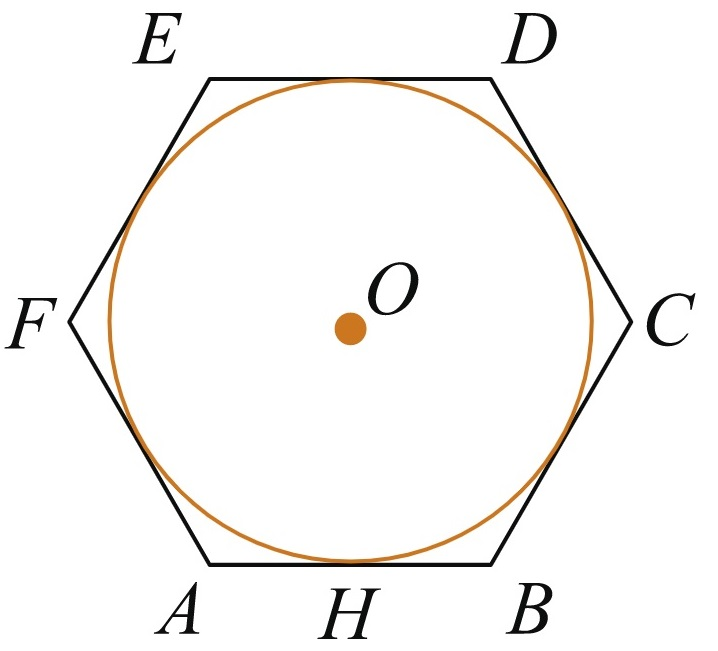
\includegraphics[align=t, width=\linewidth]{\picpath/MECGERM9H3-1}
		\end{minipage}
		\item
		\begin{minipage}[t]{\bodywidth}
			Сторона правильного треугольника равна \(\sqrt{3}\). Найдите радиус окружности, вписанной в этот треугольник.
		\end{minipage}
		\hspace{0.02\linewidth}
		\begin{minipage}[t]{\picwidth}
			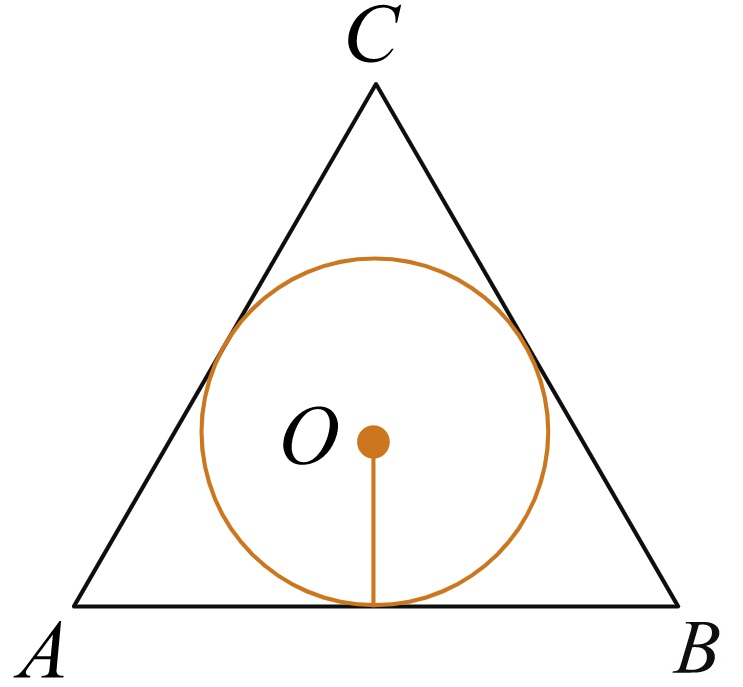
\includegraphics[align=t, width=\linewidth]{\picpath/MECGERM9H3-2}
		\end{minipage}
		
		\item
		\begin{minipage}[t]{\bodywidth}
			Через концы \(A, B\) дуги окружности в \(62\degree \) проведены касательные \(AC\) и \(BC\). Найдите угол \(ACB\). Ответ дайте в градусах.
		\end{minipage}
		\hspace{0.02\linewidth}
		\begin{minipage}[t]{\picwidth}
			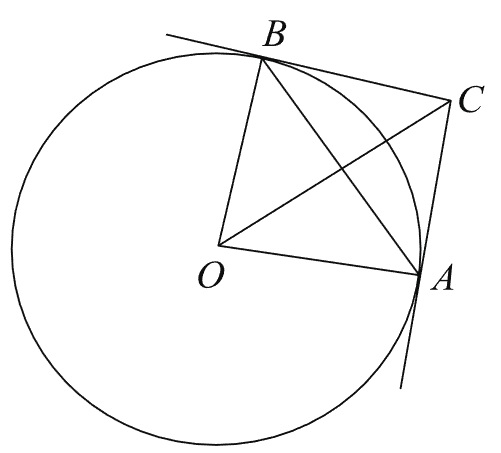
\includegraphics[align=t, width=\linewidth]{\picpath/MECGERM9H2-5}
		\end{minipage}
		%\item На экзамен вынесено \(60\) вопросов, Андрей не выучил \(3\) из них. Найдите вероятность того, что ему попадется выученный вопрос.
		%\item В среднем из \(1400\) садовых насосов, поступивших в продажу, \(7\) подтекают. Найдите вероятность того, что один случайно выбранный для контроля насос не подтекает.
		%\item Фабрика выпускает сумки. В среднем \(8\) сумок из \(100\) имеют скрытые дефекты. Найдите вероятность того, что купленная сумка окажется без дефектов.
		%\item При производстве в среднем на каждые \(2982\) исправных насоса приходится \(18\) неисправных. Найдите вероятность того, что случайно выбранный насос окажется неисправным.
		%\item Какова вероятность того, что случайно выбранный телефонный номер оканчивается двумя чётными цифрами?
		\newpage
		\item Если шахматист \(A\) играет белыми фигурами, то он выигрывает у шахматиста \(B\) с вероятностью \(0,52\). Если \(A\) играет черными, то \(A\) выигрывает у \(B\) с вероятностью \(0,3\). Шахматисты \(A\) и \(B\) играют две партии, причём во второй партии меняют цвет фигур. Найдите вероятность того, что \(A\) выиграет оба раза.
		
		%\item Симметричную монету бросают \(10\) раз. Во сколько раз вероятность события "выпадет ровно \(5\) орлов" больше вероятности события "выпадет ровно 4 орла"?
		%\item В одном ресторане в г. Тамбове администратор предлагает гостям сыграть в "\textbf{Шеш-беш}": гость бросает одновременно две игральные кости. Если он выбросит комбинацию \(5\) и \(6\) очков хотя бы один раз из двух попыток, то получит комплимент от ресторана: чашку кофе или десерт бесплатно. Какова вероятность получить комплимент? Результат округлите до сотых.
		
		
	\end{listofex}
\end{class}
%END_FOLD

%BEGIN_FOLD % ====>>_ Проверочная работа _<<====
\begin{class}[number=8]
	\begin{listofex}
		%11vpis 1 3 6 8
		\item Периметр треугольника равен \(76\), а радиус вписанной окружности равен \(8\). Найдите площадь этого треугольника.
		\item Найдите радиус окружности, вписанной в правильный треугольник, высота которого равна \(6\).
		\item Сторона правильного треугольника равна \(\sqrt{3}\). Найдите радиус окружности, вписанной в этот треугольник.
		\item Сторона ромба равна \(1\), острый угол равен \(30\) градусов. Найдите радиус вписанной окружности этого ромба.
		\item Катеты равнобедренного прямоугольного треугольника равны \(2+\sqrt{2}\). Найдите радиус окружности, вписанной в этот треугольник.
		%11.4 5 6 po 19-21
		\item Найдите наименьшее значение функции \( y=(x^2-8x+8)e^{2-x} \) на отрезке \( [1;7] \).
		%\item Найдите наибольшее значение функции \( y=(x^2-10x+10)e^{10-x} \) на отрезке \( [5;11] \).
		\item Найдите наибольшее значение функции \( y=(x-2)^2e^{x-2} \) на отрезке \( [1;4] \).
		\item Найдите точку максимума функции \( y=2\ln(x+4)^3-8x-19 \).
		%\item Найдите точку максимума функции \( y=0,5x^2-7x+12\ln x+8 \).
		%\item Найдите наименьшее значение функции \( y=4x^2-10x+2\ln x-5 \) на отрезке \( [0,3;3] \).
		\item Найдите наибольшее значение функции \( y=7\cos x+16x-2 \) на отрезке \( \left[ -\dfrac{ 3\pi }{ 2 };0 \right] \).
		%\item Найдите наименьшее значение функции \( y=13x-9\sin x+9 \) на отрезке \( \left[ 0;\dfrac{ \pi }{ 2 } \right] \).
		\item Найдите точку максимума функции \( y=(2x-3)\cos x - 2 \sin x+5 \), принадлежащую промежутку \( \left( 0; \dfrac{ \pi }{ 2 } \right) \).
		%\item Монету подбрасывают \(8\) раз. Найдите математическое ожидание количества выпавших орлов.
		%\item Монету подбрасывают до тех пор, пока орёл не выпадет два раза (не обязательно подряд). Найдите математическое ожидание числа бросков.
		%\item В торговом центре два одинаковых автомата продают кофе. Обслуживание автоматов происходит по вечерам после закрытия центра. Вероятность события "К вечеру в первом автомате закончится кофе" равна \(0,2\). Вероятность события "К вечеру в втором автомате закончится кофе" равна \(0,6\). Считая эти события независимыми, найдите математическое ожидание числа автоматов, в которых к вечеру закончится кофе.
		%\item Игральную кость бросали до тех пор, пока сумма всех выпавших очков не превысила число \(3\). Какова вероятность того, что для этого потребовалось ровно два броска? Ответ округлите до сотых.
		\item При изготовлении подшипников диаметром \(67\) мм вероятность того, что диаметр будет отличаться от заданного не больше, чем на \(0,01\) мм, равна \(0,965\). Найдите вероятность того, что случайный подшипник будет иметь диаметр меньше чем \(66,99\) мм или больше чем \(67,01\) мм.
		\item Вероятность того, что в случайный момент времени температура тела здорового человека окажется ниже чем \(36,8 \degree C\), равна \(0,81\). Найдите вероятность того, что в случайный момент времени у здорового человека температура окажется \(36,8 \degree C\) или выше.
		\item В магазине стоят два платёжных автомата. Каждый из них может быть неисправен с вероятностью \(0,05\) независимо от другого автомата. Найдите вероятность того, что хотя бы один автомат исправен.
		\item В торговом центре два одинаковых автомата продают кофе. Вероятность того, что к концу дня в автомате закончится кофе, равна \(0,3\). Вероятность того, что кофе закончится в обоих автоматах, равна \(0,12\). Найдите вероятность того, что к концу дня кофе останется в обоих автоматах.
		\item Вероятность того, что на тестировании по биологии учащийся \(O\) верно решит больше \(11\) задач, равна \(0,67\). Вероятность того, что \(O\) верно решит больше \(10\) задач, равна \(0,74\). Найдите вероятность того, что \(O\) верно решит ровно \(11\) задач.
		
		
		
	\end{listofex}
\end{class}
%END_FOLD

%BEGIN_FOLD % ====>>_____ Занятие 6 _____<<====
\begin{homework}[number=4]
	\begin{listofex}
		\item Найдите наименьшее значение функции \( y=(x^2-8x+8)e^{2-x} \) на отрезке \( [1;7] \).
		%\item Найдите наибольшее значение функции \( y=(x^2-10x+10)e^{10-x} \) на отрезке \( [5;11] \).
		%\item Найдите наибольшее значение функции \( y=(x-2)^2e^{x-2} \) на отрезке \( [1;4] \).
		\item Найдите точку максимума функции \( y=2\ln(x+4)^3-8x-19 \).
		%\item Найдите точку максимума функции \( y=0,5x^2-7x+12\ln x+8 \).
		%\item Найдите наименьшее значение функции \( y=4x^2-10x+2\ln x-5 \) на отрезке \( [0,3;3] \).
		%\item Найдите наибольшее значение функции \( y=7\cos x+16x-2 \) на отрезке \( \left[ -\dfrac{ 3\pi }{ 2 };0 \right] \).
		\item Найдите наименьшее значение функции \( y=13x-9\sin x+9 \) на отрезке \( \left[ 0;\dfrac{ \pi }{ 2 } \right] \).
		\item Найдите точку максимума функции \( y=(2x-3)\cos x - 2 \sin x+5 \), принадлежащую промежутку \( \left( 0; \dfrac{ \pi }{ 2 } \right) \).
		\item При изготовлении подшипников диаметром \(67\) мм вероятность того, что диаметр будет отличаться от заданного не больше, чем на \(0,01\) мм, равна \(0,92\). Найдите вероятность того, что случайный подшипник будет иметь диаметр меньше чем \(66,99\) мм или больше чем \(67,01\) мм.
		\item Помещение освещается фонарём с двумя лампами. Вероятность перегорания лампы в течение года равна \(0,3\). Найдите вероятность того, что в течение года хотя бы одна лампа не перегорит.
		\item Радиус окружности, описанной около прямоугольного треугольника, равен \(4\). Найдите гипотенузу этого треугольника.
		\item Найдите радиус окружности, описанной около прямоугольного треугольника, если его сторона равна \(3\).
		\item В треугольнике \(ABC\) \(AC = 4, BC = 3,\) угол \(C\) равен \(90\degree \). Найдите радиус описанной окружности этого треугольника.
		\item Площадь треугольника равна \(24\), а радиус вписанной окружности равен \(2\). Найдите периметр этого треугольника.
		\item В треугольнике \(ABC\) известно, что \(AC = 36\), \(BC = 15\), а угол \(\angle C=90\) градусов. Найдите радиус вписанной в этот треугольник окружности.
		\item Один острый угол прямоугольного треугольника в \( 4 \) раза больше другого. Найдите больший острый угол. Ответ дайте в градусах.
		\item В треугольнике \(ABC\) угол \(C\) равен \(90 \degree \), \(AC=4,8\), \(\sin{A} = \dfrac{7}{25}\). Найдите \(AB\).
		\item В треугольнике \(ABC\) угол \(C\) равен \(90 \degree \), \(CH\) --- высота, \(BC=3\), \(\sin{A} = \dfrac{1}{6}\). Найдите \(AH\).
		\item Радиус окружности равен \(1\). Найдите величину острого угла, опирающегося на хорду \(\sqrt{3}\).
		%\item
		%\begin{minipage}[t]{\bodywidth}
		%	Найдите площадь четырехугольника, изображенного на клетчатой бумаге с размером клетки \(1 \times 1\) см (см. рис.). Ответ дайте в квадратных сантиметрах.
		%\end{minipage}
		%\hspace{0.02\linewidth}
		%\begin{minipage}[t]{\picwidth}
		%	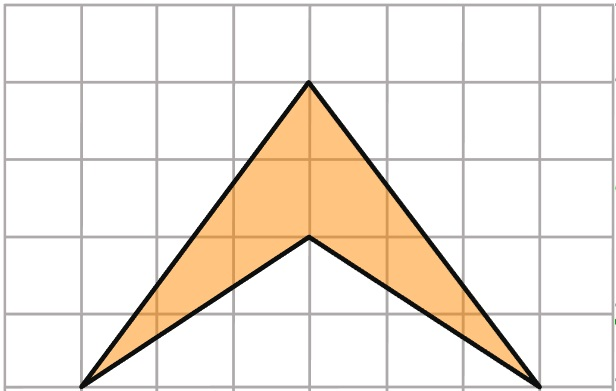
\includegraphics[align=t, width=\linewidth]{\picpath/G111M9H4-1}
		%\end{minipage}
		%\item
		%\begin{minipage}[t]{\bodywidth}
		%	Найдите площадь четырехугольника, изображенного на клетчатой бумаге с размером клетки \(1 \times 1\) см (см. рис.). Ответ дайте в квадратных сантиметрах.
		%\end{minipage}
		%\hspace{0.02\linewidth}
		%\begin{minipage}[t]{\picwidth}
		%	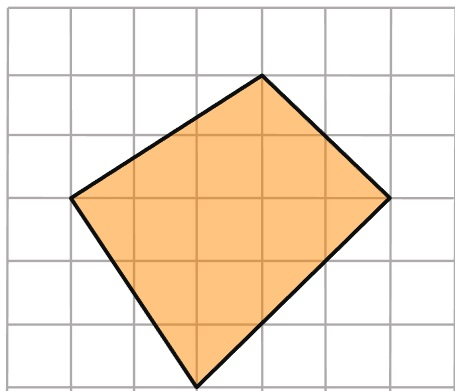
\includegraphics[align=t, width=\linewidth]{\picpath/G111M9H4-2}
		%\end{minipage}
		%\item
		%\begin{minipage}[t]{\bodywidth}
		%	Найдите площадь прямоугольника, изображенного на клетчатой бумаге с размером клетки \(1 \times 1\) см (см. рис.). Ответ дайте в квадратных сантиметрах.
		%\end{minipage}
		%\hspace{0.02\linewidth}
		%\begin{minipage}[t]{\picwidth}
		%	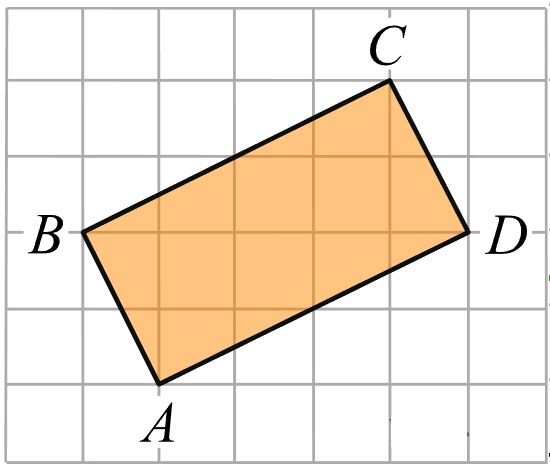
\includegraphics[align=t, width=\linewidth]{\picpath/G111M9H4-3}
		%\end{minipage}
	\end{listofex}
\end{homework}
%END_FOLD